%webimpl.tex
This section describes the work of implementing the web interface in Servlets.

\subsubsection{Requirements}
\label{subsec:webReq}
The requirements for the web interface have been gathered from the other project groups, and are as follows:
\begin{description}
	\item[Profile management] It must be possible to add, edit and remove users.
	\item[Media management] It must be possible to add, edit and remove media, add tags, and link pictures and sound.
	\item[Settings] It must be possible to add and change the settings for a specific user.
	\item[Stats] It must be possible to generate stats of the use of various apps.
\end{description}

\subsubsection{Mockups}
To get started, a series of mockups were created to get an idea of the general look and feel of the website. An example of this is shown in \autoref{fig:mockSelectProfile}, the rest can be found in \autoref{app:Mock}.

\begin{figure}[htbp]
	\centering
		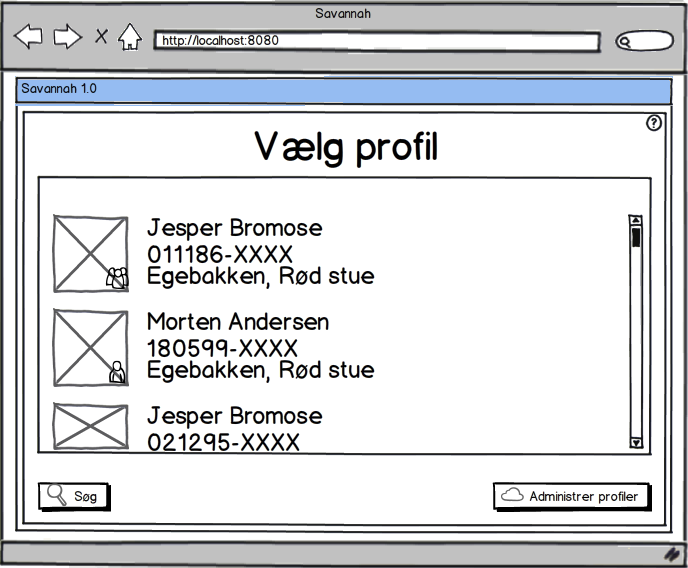
\includegraphics[width=1.00\textwidth]{images/mockSelectProfile.png}
	\caption{A mockup of profile selection}
	\label{fig:mockSelectProfile}
\end{figure}

\subsubsection{Programming languages}
The web interface uses four different languages: Servlets, HTML, JavaScript, and Cascading Style Sheets (CSS). The Servlets are responsible for database access, and generation of both the HTML code and JavaScript, and the CSS is used for the layout on each page. The HTML is used for making the elements on the webpages, and the JavaScript is used to add functionality to a generated HTML page.

\subsubsection{Structure}
The structure of each Servlet is seen in \autoref{fig:webStruct}
\begin{figure}
	\centering
		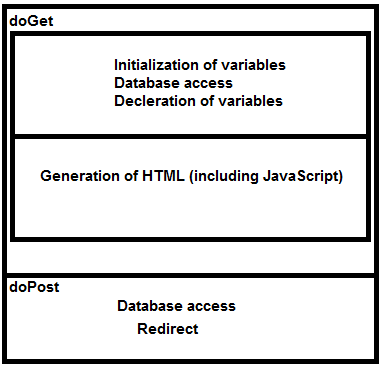
\includegraphics{images/webStruct.png}
	\caption{General structure of Servlets}
	\label{fig:webStruct}
\end{figure}

When a webpage is first loaded, it execute the \code{doGet(...)} method. After this there are three scenarios:
\begin{description}
	\item[Scenario 1] The user clicks a link, and is sent to a new page.
	\item[Scenario 2] The user submits a \code{form} with the \code{doGet(...)} method. 
	\item[Scenario 3] The user submits a \code{form} with the \code{doPost(...)} method.
\end{description}

In scenario 1, the current page does not do anything else but send the user to the new page, which executes the code in its \code{doGet(...)} method. In scenario 2, the \code{form} structure dictates what happens: It can either redirect to itself, and execute the \code{doGet(...)} method again, see \autoref{code:getRedirectSelf}, or redirect to a new page and execute the \code{doGet(...)} method on that page, see \autoref{code:getRedirectNew}.

\begin{lstlisting}[language=Java,label=code:getRedirectSelf,caption=A \code{form} which redirect to its own get method]
	@WebServlet("/DeleteTags")
	
	/**
	 * @see HttpServlet#doGet(HttpServletRequest request, HttpServletResponse response)
	 */
	protected void doGet(HttpServletRequest request, HttpServletResponse response) throws ServletException, IOException {
	
	out.println("<center><form method='GET' name='formName' action='DeleteTags'>");
	}
\end{lstlisting}

\begin{lstlisting}[language=Java,label=code:getRedirectNew,caption=A \code{form} which redirect to another page]
	@WebServlet("/DeleteTags")
	
	/**
	 * @see HttpServlet#doGet(HttpServletRequest request, HttpServletResponse response)
	 */
	protected void doGet(HttpServletRequest request, HttpServletResponse response) throws ServletException, IOException {
	
	out.println("<center><form method='GET' name='formName' action='NewPage'>");
	}
\end{lstlisting}

Scenario 3, has almost the same code as \autoref{code:getRedirectSelf} and \autoref{code:getRedirectNew}, with the exception that the \code{method='POST'}.

In general the \code{form} is build as \code{<form method='POST/GET' name='NameOfForm' action='WhichPageToExecuteCodeFrom>}.

\subsubsection{Database Access}
Reading data from the database is handled by Java code in each of the Servlets, shown in \autoref{code:readDatabase}.
To update attributes in the database, the \code{stmt.executeQuery(``SQL query'')} method is used, with the appropriate SQL script.
To delete data, instead of \code{stmt.executeQuery(``SQL query'')} a \code{PreparedStatement} is created, this is executed with by calling \code{int i = ps.executeUpdate()} which will return a response code. 

\begin{lstlisting}[language=Java,label=code:readDatabase,caption=Code to read data from the database]
public void readData()
{
String dataVar;
Connection con = null;
Statement stmt = null;
ResultSet rs = null;
try {
   Class.forName("com.mysql.jdbc.Driver"); //Use this driver to access the database
   con = DriverManager.getConnection("jdbc:mysql://DatabaseAddress", "Username", "Password"); //Instansiate the connection
   stmt = con.createStatement(); //Instansiate stmt
   rs = stmt.executeQuery("SQL query"); //Executes the SQL query and get the result store in RS
   //As long rs contains data, read it!
   while (rs.next()) { 
      String name = rs.GetString("Name"); //Get a string attribute
      int number = rs.GetString("Number"); //Get a int attribute
}
//Error handeling
catch (SQLException e) 
{		
   throw new ServletException("Servlet Could not display records.", e);
} 
catch (ClassNotFoundException e) 
{			
   throw new ServletException("JDBC Driver not found.", e);
}
//Make sure the connection is closed, no matter what 
finally {
   try {
      if (rs != null) {
         rs.close();
         rs = null;
      }
      if (stmt != null) {
         stmt.close();
         stmt = null;
      }
      if (con != null) {
         con.close();
         con = null;
      }
   } 
catch (SQLException e) 
{			
}
}

\end{lstlisting}

\subsubsection{Generation of a Web Page}
The generation of a web page, is done within the Servlet, using a \code{PrintWriter}. This is used to write the HTML code by calling \code{out.println("HtmlCode")} which appends the argument to the page. Furthermore, \code{out} can be used to write both JavaScript and CSS.

The CSS is not written within any of the Servlets, instead it is located in a separate file and is included in the HTML by \code{ out.println("<link rel='stylesheet' type='text/css' href='CSS/SavannahStyle.css' />")}.

\subsubsection{Exchange of Data}
When a Servlet submits a form, the data is sent differently depending on the \code{<form method='...'/>}. A \code{GET} will send the data as a part of the URL, thus making it visible for the user, as seen in \autoref{code:URLLINK}, whereas the \code{POST} method does not make it visible.

\subsubsection{Form Data}
To access the data from the \code{form}, the elements in the \code{form} needs a name. The name is set by the \code{name} attribute in the input element. The type of data sent from the \code{form} depends on the type of element.
\begin{description}
	\item[Text/Password] seen in \autoref{code:HTMLTxt}. The value of these fields are of the type string, and contains the value entered into the text field on the page.
	\item[RadioButton] seen in \autoref{code:HTMLradi}. All \code{RadioButton}s with the same name, sends \code{some_value} of the selected \code{RadioButton}.
	\item[CheckBox] seen in \autoref{code:HTMLcheck}. All \code{CheckBox}es with the same name sends \code{some_value} of each checked box.
	\item[DropDown menu] seen in \autoref{code:HTMLdrop}. Sends \code{some_value} of the selected item.
	\item[Multiple Select] seen in \autoref{code:HTMLmulSel}. Sends \code{some_value} of all the selected items as a string array.
\end{description}

\begin{lstlisting}[language=Java,label=code:URLLINK,caption=URL with visible parameters]
http://www.xoxoxoxox.com/servlet/ServletName?var1=value&var2=value&var3=value
\end{lstlisting}

To be able to retrieve the data sent by the form the \code{request.getParameter()} method is used. An example of this is shown in \autoref{code:getDataInPost}.

\begin{lstlisting}[language=Java,label=code:getDataInPost,caption=How to read parameters]
	@WebServlet("/PseudoClass")
	/**
	 * @see HttpServlet#doPost(HttpServletRequest request, HttpServletResponse response)
	 */
	protected void doPost(HttpServletRequest request, HttpServletResponse response) throws ServletException, IOException {
		String myVar = request.getParameter("FieldName"); //Get single Value
		String[] myVarArray = request.getParameterValues("FieldName") //Get string array
	}
\end{lstlisting}

\subsubsection{Current limitatio}
When uploading a picture, a \code{file} type is used to select the local file on the hard disk. The \code{file} has a security restricting, which makes it impossible to set a default value for the field. This is due to the fact, that if it was possible, it could be used to send a file from the visitor of a web page's hard disk, without the visitor has any knowledge of it\cite{noFile}. Futhermore it was not straight forward to get the path of a selected file, again due to security restrictions, but this turned out to be possible by the use of JavaScript, the code is seen in \autoref{code:myHack}, and adding parameter \code{onChange="readURL(this);"} to the \code{file} field.

\begin{lstlisting}[language=HTML,label=code:myHack,caption=Hack to load file from \code{file} box]
var reader = new FileReader();+
reader.onload = function(e) 
   {
      document.billedet.src  = e.target.result;
   };

function readURL(input)
   {
      if(input.files && input.files[0])
      {
         reader.readAsDataURL(input.files[0]);
      }
      else 
      {
         document.billedet.src = "";
      }
   }
\end{lstlisting}

A navigation diagram of the web site is shown in \autoref{fig:WebNav}, and shows that all pages and information can be accessed within three clicks.

\begin{figure}
	\centering
		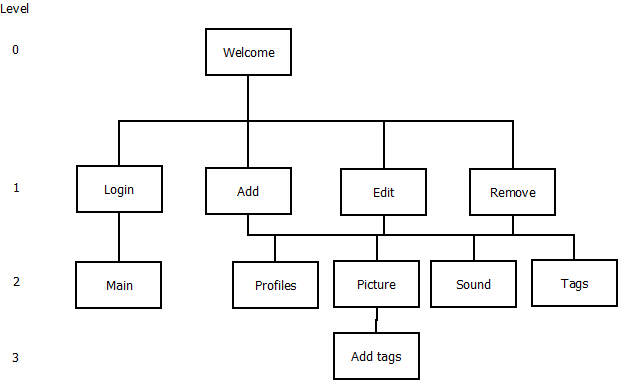
\includegraphics[width=1.00\textwidth]{images/WebNav.png}
	\caption{Navigation diagram for the web site}
	\label{fig:WebNav}
\end{figure}
